\section{Results and Discussion} \label{sec:results}

This section begins by assessing the newly proposed surface-based hereditary stratigraphy algorithms against the existing column-based algorithms in terms of their semantic behavior (how does what data they store influence reconstruction accuracy?) and implementation efficiency (how much time does one annotation update take?).
Then, we report results of an experiment validating end-to-end application of the implementation of the tilted surface algorithm for the Cerebras Software Language on the WSE hardware emulator.

Next, we report benchmarking experiments for the asynchronous island-model genetic algorithm implemented for the WSE platform, also conducted on the hardware emulator.
Finally, we show example phylogenies generated from on-hardware simulations under different selection pressure conditions and test the capability of inference from extracted phylogenetic information to detect differing selection pressure conditions.

\subsection{Reconstruction Quality of New Surface Algorithms}

\begin{figure*}
  \centering
  \includegraphics[width=\textwidth]{binder-reconstruction-quality/binder/surf-vs-col/outplots/surf-vs-col-table}
  \caption{%
   \textbf{Comparison of reconstruction accuracies from column- and surface-based annotations.}
    Color coding represents non-parametric difference between accuracy measures, with red indicating superior surface performance and blue indicating superior column performance.
    Left column shows tilted retention policies, and right column shows steady retention policies.
    For heatmap charts, +'s indicate small, medium, and large effect sizes using the Cliff's delta statistic and *'s indicate statistical significance at $\alpha = 0.05$ via Mann-Whitney U test.
  }
  \label{fig:col-vs-surf}
\end{figure*}


Figure \ref{fig:col-vs-surf} compares reconstruction quality for surface algorithms against their corresponding column implementation.
We did this by using a simple simulation to generate phylogenies under different conditions with perfect tracking, then simulating heritage of hstrat annotations down the perfect tree and subsequent reconstruction.
We could then compare the reconstruction that would have been obtained under approximate tracking to the underlying ground truth.

To ensure generalizable results, we tested over a large number of evolutionary regimes, population sizes, instrumentation sizes, and instrumentation fingerprint sizes.
Each row in Figure \ref{fig:col-vs-surf} represents a distinct combination of surveyed conditions.

We took three measures of reconstruction quality.
The first measure, triplet distance, is a measure of accuracy --- it is the fraction of triplet tips that are correctly arranged in the reconstruction.
Whereas this metric considers polytomies as distinct from separate branching events, our second measure is a lax variant of triplet distance that does not penalize penalties introduced into the reconstruction (i.e., due to uncertainty about branching order) or over-resolution of true polytomies into more nodes in the reconstruction.
Finally, we also include inner node count, which provides a measure of the amount of detail achieved by reconstructions.
Higher inner node count indicates that fewer branching events are being lumped together into polytomies due to insufficient information to differentiate them.
This metric is only applicable to scenarios with fingerprint sizes larger than one bit (i.e., a byte), which are capable of generating non-bifurcating trees.

The data tell two clear stories:
\begin{enumerate}
\item surface tilted algorithms create higher-quality reconstructions than column-based tilted algorithms and
\item surface column algorithms create lower-quality reconstructions than column-based column algorithms.
\end{enumerate}

The surface tilted performs significantly best in 14 / 48 scenarios for triplet distance, 9 / 48 for lax triplet distance, and all scenarios where inner node count is applicable.
It performs significantly worse in no scenarios.

The surface steady performs significantly worse in 11 / 48 scenarios for triplet distance, in 1/48 scenarios for lax triplet distance, and 4/12 scenarios for inner node loss.
The surface steady performs significantly better than the column in no scenarios.

The performance advantage of surface-tilted is likely because the surface-based algorithms can make better use of available space --- every site is always in use to store a fingerprint.
In contrast, under the column-based approach, some fraction of the available space is typically unused because of difficulty predicting the order with which sites will need to be eliminated \textit{a priori} and thus eliminating them based on a heuristic (TODO rewrite this sentence).

The performance detriment of column-steady likely stems from precise control of the column approach to sequence eliminations.
The surface approach guarantees adherence to the fixed resolution qualities provided by the column approach, but the process of degrading from one spacing to the next double-width spacing is slightly more irregular on account of the additional consideration of being mapped onto the surface.
Unlike the tilted algorithm, the steady column algorithm does not have difficulty filling available space.

Recent work indicates that tilted policies should be preferred for better reconstruction accuracy in most cases, except where there are extreme factors promoting phylogenetic richness.
Thus, degraded reconstruction performance from the steady surface is not much of a concern because the steady policy is not expected to be used frequently in practice.
So, in addition to being capable of being implemented in a broader range of device contexts (not needing memory allocation or rich data structures) and being faster to calculate (discussed next), the surface-based approach can provide higher-quality phylogenetic reconstructions.

\subsection{Surface Algorithm Benchmark}

\begin{figure*}
  \centering
  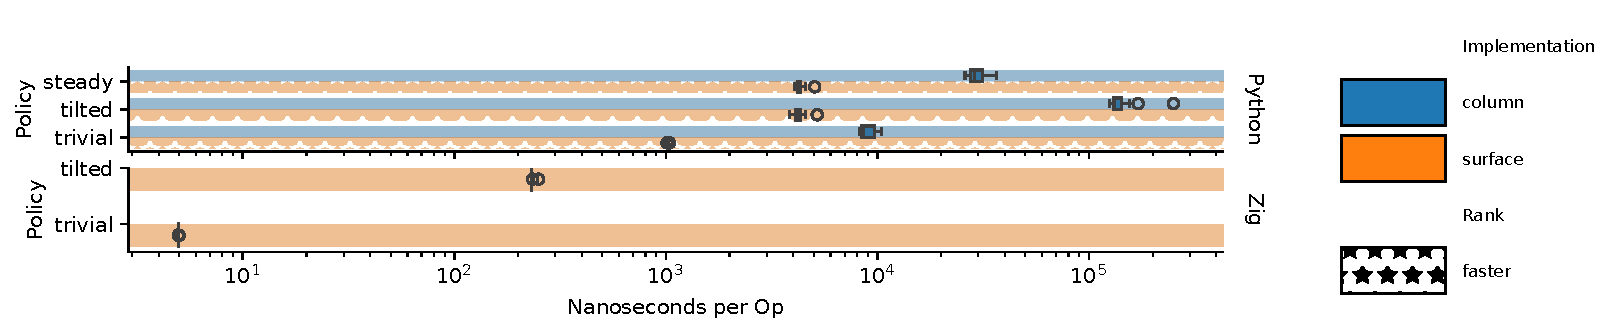
\includegraphics[width=\textwidth]{binder-wafer-scale/binder/teeplots/all=false+hue=implementation+orient=h+row=language+score=nanoseconds-per-op+viz=peckplot+x=nanoseconds-per-op+y=policy+y-group=outer+ext=}

\vspace{-2.5ex}

  \caption{%
    \textbf{Hereditary stratigraphy algorithm benchmarks.}
    \footnotesize
    Comparison of per-generation operation time for column- and surface-based steady and tilted retention policies, lower is better.
  Top and bottom panels show Python and Zig implementations, respectively.
    Trivial is a simple harcoded retention decision, provided as a baseline control.
    Background hatching indicates significant outcome (Mann-Whitney U test; $n=20$).
  }
  \label{fig:benchmarking}
  \vspace{-0.2in}
\end{figure*}


We performed benchmarking experiments to assess the computational performance of our new surface-based algorithms.
Due to limited completed implementations of compiled-language algorithms, we performed the bulk of benchmarking using the Python implementations.
While Python is an interpreted language and the Python-implemented algorithms weren't specifically implemented to maximize performance and suffer an intrinsic performance penalty due to that, the algorithms were all on the same footing and we use the ``optimize''' flag to strip assert statements out of the benchmarks.
However, in the process of porting the tilted surface algorithm over to Cerebras Software Language, we did create an implementation of that algorithm in Zig which is a compiled language and is capable of compiler optimizations.
We augment the Python with a benchmark of this algorithm.
Figure \ref{fig:benchmarking} provides an overview of the results.

% https://github.com/mmore500/hstrat-surface-concept/blob/51d636d768d474fc5148b9fcaa199c1b7776e915/benchmark.ipynb
We found that the Python implementations of the surface tilted and steady algorithms both took around 4,200ns per operation (SEM c. 50; $n=20$).
For context, this was about $4\times$ the measured time for a surface placement using a trivial calculation (SEM c. 0.05; $n=20$).
The column implementations of steady and tilted fared much worse, taking about $7\times$ and $34\times$ the execution time per operation compared to the surface operations.
Mann-Whitney U tests confirmed that surface implementations significantly outperformed their column counterparts. (Figure \ref{fig:benchmarking}).

% https://github.com/mmore500/wse-sketches/blob/d4ab0155f63ff5809f8eeca1169ad9b272c30a68/binder/benchmark.ipynb
Zig implementation of tilted surface:
233 ns per operation (SEM 0.9; $n=20$).
This was $47\times$ the measured time for a trivial placement calculation (SEM 0.2; $n=20$).
For context, this time a little more than twice the amount of time required for a main memory access in contemporary computing hardware \citep{markus2022memory}.

Note that further speedups and optimizations can likely to be had.
For single-bit differentiae, half of the time placement need not be calculated if the coin flip indicates that the bit isn't going to be flipped.
Further, in synchronous and near-synchronous simulations, placement positions can be cached meaning they would only need to be calculated once for an entire subpopulation.

\subsection{WSE Hereditary Stratigraphy Validation Experiment}

We performed extensive tests to be confident in our implementation of phylogenetic tracking for the Cerebras Software Language on the WSE device.
Extensive other work TODOCITE has validated the underlying hereditary surface algorithm and the reconstruction algorithm.
We also used extensive unit tests in CSL to ensure the algorithm was working as expected.

Here, we report the results of an integration test to assess the general validity of phylogenetic reconstructions on the WSE platform.
We used special genomes tagged with a randomly-generated identifier at simulation startup.
Figure \ref{fig:genome-layout} explains the content laid out within each genome.
These identifiers identified clades descending from each founding genome.
We used the hardware simulator to perform a simulation on the $3\times3$ PE collective under drift conditions for 25, 50, 100, and 250 generation cycles.

\begin{figure*}

\begin{subfigure}[c]{\textwidth}
\begin{minipage}[c]{0.1\textwidth}
    \caption{25 cycles}
    \label{fig:tagged_25}
  \end{minipage}
  \begin{minipage}[c]{0.9\textwidth}
    \includegraphics[width=\textwidth,height=0.8in,trim={0 0.81cm 0 0},clip]{binder-wse-sketches/binder/teeplots/genome=hsurftiltedsticky_tagged+replicate=e4ea2071-8228-42de-af8c-879cedff9ba7+viz=draw-biopython-tree+ext=}
  \end{minipage}
\end{subfigure}

\vspace{-1ex}

\begin{subfigure}[c]{\textwidth}  \begin{minipage}[c]{0.1\textwidth}
    \caption{50 cycles}
    \label{fig:tagged_50}
  \end{minipage}
  \begin{minipage}[c]{0.9\textwidth}
    \includegraphics[width=\textwidth,height=0.8in,trim={0 0.81cm 0 0},clip]{binder-wse-sketches/binder/teeplots/genome=hsurftiltedsticky_tagged+replicate=3d55af5f-7714-45da-9276-e860f46b4d94+viz=draw-biopython-tree+ext=}
  \end{minipage}
\end{subfigure}

\vspace{-1ex}

\begin{subfigure}[c]{\textwidth}
  \begin{minipage}[c]{0.1\textwidth}
    \caption{100 cycles}
    \label{fig:tagged_100}
  \end{minipage}
  \begin{minipage}[c]{0.9\textwidth}
    \includegraphics[width=\textwidth,height=0.8in,trim={0 0.81cm 0 0},clip]{binder-wse-sketches/binder/teeplots/genome=hsurftiltedsticky_tagged+replicate=932aa302-becb-47e8-9712-7f550b02364c+viz=draw-biopython-tree+ext=}
  \end{minipage}
\end{subfigure}

\vspace{-1ex}

\begin{subfigure}[c]{\textwidth}
  \begin{minipage}[c]{0.1\textwidth}
    \caption{250 cycles}
    \label{fig:tagged_250}
  \end{minipage}
  \begin{minipage}[c]{0.9\textwidth}
    \includegraphics[width=\textwidth,height=1in]{binder-wse-sketches/binder/teeplots/genome=hsurftiltedsticky_tagged+replicate=42dbcbb3-b803-41a4-9285-4a450bfad6ed+viz=draw-biopython-tree+ext=}
  \end{minipage}
\end{subfigure}

\caption{%
\textbf{Clade Validation Trial.}
Example phylogenies reconstructed from runs of increasing duration on virtual grid of nine hardware-simulated PEs.
Founding genomes were tagged with random 16-byte identifier values, which were held constant over the course of simulation (Supplementary Figure \ref{fig:genome-layout}).
Color-coding indicates each sampled taxon's founding ancestor according to this identifier value.
Simulation performed under drift conditions.
}
\label{fig:tagged}

\end{figure*}


Figure \ref{fig:tagged} shows reconstructed phylogenies from each duration.
As expected, taxa belonging to the same founding clade are reconstructed as more closely related than to other taxa and the number of distinct founding clades represented dwindles with increasing simulation duration.

At the end of simulation, one genome was sampled per PE.
Figure \ref{fig:validation-example:phylogeny} shows the result of phylogenetic reconstruction on these sampled genomes.
To simplify visualization of the phylogeny with existing phyloinformatic tools, all clades were stitched together into a single tree by attaching them to a common ancestor.
Taxa are colored according to their clade genesis tag.
Clade arrangement in the reconstructed tree agrees well with founding clade identities.
All different-colored taxa are predicted to have had ancient common ancestry.
Note that relatedness between \texttt{0x5fb} and \texttt{0xde40} is slightly overestimated, due to a configured lack of precise resolution necessary to ensure compact genetic annotations.
Applications where high reconstruction precision is required can opt to use larger annotation sizes.


\subsection{WSE Genetic Algorithm Benchmark}

We used the cycle counter on the WSE hardware simulator to test the amount of real time elapsed over the course of a 100 generation cycle simulation on a $3\times3$ PE collective with the tagged 3 word genome, applying a tilted hereditary stratigraphy every generation.

Each PE completed a mean of 29,500 generation cycles per second (SEM 155; $n=9$), or around 2 billion generations a day.
Over the course of the simulation, each PE immigrated a mean of 277 genomes (SEM 23; $n=9$).

How would this look on a full piece of hardware?
Keeping 32 individuals per PE would result in a net population size of around 27 million on a full WSE.
(Although generation time would be slower, available memory on the CS-2 could support on the order of thousands of agents per PE potentially yielding a net population size on the order of a billion agents.)
% 29,500 * 850,000 * 60 * 60 * 24 * 32 ---> 69 quadrillion
Naive extrapolation would estimate on the order of a quadrillion agent replications every half hour, notwithstanding scaling slowdown.

% https://github.com/mmore500/wse-sketches-mirror/actions/runs/8546407499/job/23416697013
% from https://github.com/mmore500/wse-sketches-mirror/commit/fb7f9c4e175818253f844909297d747cd813b9c7
% Reading file out/out.json
% Reading file out/bin/out_rpc.json
% Reading file out/west/out.json
% Reading file out/east/out.json
% fab w,h = 10,5
% Kernel x,y w,h = 4,1 3,3
% memcpy x,y w,h = 1,1 8,3
% ASYNC_GA_GLOBAL_SEED 3
% ASYNC_GA_NCYCLE 100
% CSLC cslc
% ASYNC_GA_GENOME_FLAVOR genome_hsurftiltedsticky_tagged
% ASYNC_GA_GLOBAL_SEED 3
% ASYNC_GA_NCYCLE 100
% INFO: Using SIF: /home/runner/cerebras/bin/cbcore_sdk-202311111408-10-4a54bce5.sif
% INFO: User's specified CSL_IMPORT_PATH=
% NOTE: CSL_IMPORT_PATH accepts colon separated list of paths generated by 'realpath <path>'
% INFO:    Environment variable SINGULARITYENV_CSL_SUPPRESS_SIMFAB_TRACE is set, but APPTAINERENV_CSL_SUPPRESS_SIMFAB_TRACE is preferred
% compile successful
% Updated 1 path from the index
% CS_PYTHON cs_python
% INFO: Using SIF: /home/runner/cerebras/bin/cbcore_sdk-202311111408-10-4a54bce5.sif
% INFO:    Environment variable SINGULARITYENV_CSL_SUPPRESS_SIMFAB_TRACE is set, but APPTAINERENV_CSL_SUPPRESS_SIMFAB_TRACE is preferred
% whoami ===============================================================
% [[0 3 6]
%  [1 4 7]
%  [2 5 8]]
% whereami x ===========================================================
% [[0 1 2]
%  [0 1 2]
%  [0 1 2]]
% whereami y ===========================================================
% [[0 0 0]
%  [1 1 1]
%  [2 2 2]]
% cycle counter =======================================================
% [[100 100 100]
%  [100 100 100]
%  [100 100 100]]
% recv counter N ========================================================
% [[ 1  1  1]
%  [29 25 29]
%  [27 25 26]]
% recv counter S ========================================================
% [[23 25 25]
%  [25 27 23]
%  [ 1  1  1]]
% recv counter E ========================================================
% [[25 29  1]
%  [25 26  1]
%  [23 27  1]]
% recv counter W ========================================================
% [[ 1 23 24]
%  [ 1 23 25]
%  [ 1 25 27]]
% recv counter sum =====================================================
% [50, 78, 51, 80, 101, 78, 52, 78, 55]
% np.mean(recvSum)=69.22222222222223 np.std(recvSum)=16.857426835260856 sps.sem(recvSum)=5.960000414284516
% send counter N ========================================================
% [[100 100 100]
%  [100 100 100]
%  [100 100 100]]
% send counter S ========================================================
% [[112 102 112]
%  [108 100 104]
%  [  0   0   0]]
% send counter E ========================================================
% [[ 90 100   0]
%  [ 94 102   0]
%  [102 110   0]]
% send counter W ========================================================
% [[  0 102 112]
%  [  0 100 104]
%  [  0  92 108]]
% send counter sum =====================================================
% [202, 304, 224, 296, 404, 306, 204, 312, 202]
% np.mean(sendSum)=272.6666666666667 np.std(sendSum)=65.40812046085885 sps.sem(sendSum)=23.125262761269934
% tscControl values ====================================================
% [30064968187, 30064968187, 30064968187, 30064968187, 30064968187, 30064968187, 30064968187, 30064968187, 30064968187]
% tscStart values ======================================================
% [2623, 2137, 1653, 3133, 2648, 2114, 1627, 3111, 3111]
% tscEnd values ========================================================
% [2833350, 2958017, 2834797, 2901552, 2894748, 2906881, 2847462, 2935863, 2847357]
% tsc diffs ============================================================
% --------------------------------------------------------------- ticks
% [2830727, 2955880, 2833144, 2898419, 2892100, 2904767, 2845835, 2932752, 2844246]
% np.mean(tsc_ticks)=2881985.5555555555 np.std(tsc_ticks)=43041.3869074125 sps.sem(tsc_ticks)=15217.428276952633
% -------------------------------------------------------------- seconds
% [0.0033302670588235294, 0.0034775058823529412, 0.003333110588235294, 0.003409904705882353, 0.003402470588235294, 0.0034173729411764706, 0.003348041176470588, 0.0034502964705882353, 0.003346171764705882]
% np.mean(tsc_sec)=0.0033905712418300657 np.std(tsc_sec)=5.0636925773426534e-05 sps.sem(tsc_sec)=1.7902856796414882e-05
% ---------------------------------------------------- seconds per cycle
% [3.330267058823529e-05, 3.477505882352941e-05, 3.333110588235294e-05, 3.409904705882353e-05, 3.402470588235294e-05, 3.4173729411764705e-05, 3.348041176470588e-05, 3.4502964705882353e-05, 3.346171764705882e-05]
% np.mean(tsc_cysec)=3.390571241830066e-05 np.std(tsc_cysec)=5.063692577342663e-07 sps.sem(tsc_cysec)=1.7902856796414917e-07
% ---------------------------------------------------------- cycle hertz
% [30027.621879467715, 28756.241796013368, 30002.00483985283, 29326.332735191147, 29390.408353791365, 29262.243753113416, 29868.210911735925, 28983.016634205687, 29884.897438547865]
% np.mean(tsc_cyhz)=29500.1087046577 np.std(tsc_cyhz)=438.84515891452514 sps.sem(tsc_cyhz)=155.15519387967439
% --------------------------------------------------------- ns per cycle
% [33302.67058823529, 34775.05882352941, 33331.10588235294, 34099.04705882353, 34024.70588235294, 34173.7294117647, 33480.41176470588, 34502.964705882354, 33461.717647058824]
% np.mean(tsc_cyns)=33905.71241830065 np.std(tsc_cyns)=506.36925773426583 sps.sem(tsc_cyns)=179.028567964149
% genome values ========================================================
% ------------------------------------------------ genome binary strings
% 110101001011011001011001000000001110100101011110101001110010101000110100110101111010000000000100
% 000001111101100101011000000000001111110001111111110001100000101111101011110011001100110110110010
% 110110011001011101011101000000001010011011101000100100110001110110010000100010100111001111000101
% 001110001101110101011100000000001000110110011100000010010011100010010011110001101001011100001110
% 001110001101110101011011000000001000110100000100100000110001100000010010100000101001011100001100
% 000001111101100101100000000000001111110000100110110001111111000011110010010111101111001100100101
% 001110001101110101011011000000001100111100010101010000110011000011110110000100111011010001000101
% 000001111101100101010101000000001011110001011101100000000101010111110101110101000111010001001001
% 100110001100100101001111000000001000100110101110011111111000010001011101000001000110010001011110
% --------------------------------------------------- genome hex strings
% D4B65900E95EA72A34D7A004
% 07D95800FC7FC60BEBCCCDB2
% D9975D00A6E8931D908A73C5
% 38DD5C008D9C093893C6970E
% 38DD5B008D0483181282970C
% 07D96000FC26C7F0F25EF325
% 38DD5B00CF154330F613B445
% 07D95500BC5D8055F5D47449
% 98C94F0089AE7F845D04645E
% SUCCESS!
% Reading file out/out.json
% Reading file out/bin/out_rpc.json
% Reading file out/west/out.json
% Reading file out/east/out.json
% fab w,h = 10,5
% Kernel x,y w,h = 4,1 3,3
% memcpy x,y w,h = 1,1 8,3

\subsection{On-hardware Demonstration with Evolutionary Inference from Phylogenetic Analysis}

\begin{figure*}
  \centering
  \begin{minipage}{\textwidth}
    \centering
    Generations Ago (approx.)
  \end{minipage}
  \begin{minipage}{\textwidth}
    \hspace{0.02\linewidth}
    \rotatebox{30}{\makebox[0.1\linewidth][c]{200,000}}
    \hfill
    \rotatebox{30}{\makebox[0.1\linewidth][c]{50,000}}
    \hfill
    \rotatebox{30}{\makebox[0.1\linewidth][c]{10,000}}
    \hfill
    \rotatebox{30}{\makebox[0.1\linewidth][c]{2,000}}
    \hfill
    \rotatebox{30}{\makebox[0.1\linewidth][c]{30}}
    \rotatebox{90}{\makebox[0.04\linewidth][c]{0}}
  \end{minipage}
  \begin{subfigure}[t]{\linewidth}
    \centering
  \includegraphics[width=\linewidth,height=0.3\linewidth]{bindertex-evolutionary-inference/img/perfect-tree-phylogenies-log/epoch=7+resolution=3+treatment=22/a=collapsed-phylogeny+epoch=00007+mut_distn=np.random.standard_normal+num_generations=32768+num_islands=1024+num_niches=4+p_island_migration=0.01+p_niche_invasion=3.0517578125e-08+population_size=3276.../8+replicate=0+tournament_size=2+treatment=22+_generation=262144+_index=22+scale=log+ext=}
    \caption{%
    Tournament size 2.
    STAND-IN IMAGE.
    }
    \label{fig:wse-phylogenies-tsize2}
  \end{subfigure}

  \begin{subfigure}[t]{\linewidth}
    \centering
\includegraphics[width=\linewidth,height=0.3\linewidth]{bindertex-evolutionary-inference/img/perfect-tree-phylogenies-log/epoch=7+resolution=3+treatment=6/a=collapsed-phylogeny+epoch=00007+mut_distn=np.random.standard_normal+num_generations=32768+num_islands=1024+num_niches=1+p_island_migration=0.01+p_niche_invasion=3.0517578125e-08+population_size=3276.../8+replicate=0+tournament_size=2+treatment=6+_generation=262144+_index=6+scale=log+ext=}
    \caption{%
      Tournament size 8.
      STAND-IN IMAGE.
    }
    \label{fig:wse-phylogenies-tsize8}
  \end{subfigure}

\caption{%
\textbf{Phylogenies from on-hardware experiment.}
\footnotesize
Subfigures \ref{fig:wse-phylogenies-tsize2} and \ref{fig:wse-phylogenies-tsize8} contrast phylogenies from experiments with lower and higher selection pressure, respectively.
Note the recognizable decrease in phylogenetic richness under high selection pressure.
Each phylogeny subsampled to 131,072 taxa.
}
\label{fig:wse-phylogenies}

\end{figure*}


To perform a preliminary assessment of the practicability of this methodology in practice, we ran our genetic algorithm on a WSE device.
We annotated genomes with a 64-bit instrumentative annotation, comprising a 32-bit counter and 32-bit tilted hstrat surface.
We performed evolutionary runs under two conditions, one with tournament size 2 and one with tournament size 8.
We performed TODO replicates per condition, running each for Y minutes.
This was sufficient to observe a mean of TODO generations per cycle, SD TODO.
At the conclusion of the run, we collected one genome from each PE.

Figure \ref{fig:wse-phylogenies} compares two example reconstructed phylogenies, one from each treatment.
Performing a reconstruction with all 850,000 genomes took X minutes.
We used a Mann-Whitney U test between inner node time distributions for pairs of trees to test whether the difference in selection pressure was detectable.
Indeed, the recovered phylogenetic information was sufficient to detect this difference in evolutionary dynamics for all pairs ($p < TODO$ for all $n=TODO$).
